\documentclass[ngerman]{tudscrreprt}
\iftutex
\usepackage{fontspec}
\else
\usepackage[T1]{fontenc}
\usepackage[ngerman=ngerman-x-latest]{hyphsubst}
\fi
\usepackage{babel}
\usepackage[german]{isodate}
\usepackage{setspace}
\usepackage{float}
\usepackage{amsmath}
\usepackage{siunitx}
\usepackage{csquotes}
\usepackage[hidelinks]{hyperref}
\usepackage{multirow,tabularx}
\usepackage[center]{caption}
\newcolumntype{Y}{>{\centering\arraybackslash}X}

\newcommand{\code}[1]{\texttt{#1}}

\begin{document}
\faculty{Fakultät Maschinenwesen}
\institute{Institut für Technische Logistik und Arbeitssysteme}
\chair{Professur für Technische Logistik}
\date{2022-03-04}
\author{%
Pascal Juppe%
\matriculationnumber{4765520}%
\and%
Nico Müller%
\matriculationnumber{4765450}%
\and%
Ferdinand Thiessen%
\matriculationnumber{3977297}%
}
\title{Logistics Lab}
\subtitle{Bericht Gruppe 6}
\maketitle

% 1.25 facher Zeilenabstand
\setstretch{1.25}

% Subsection ausblenden
\setcounter{tocdepth}{1}
\tableofcontents

\chapter{Aufgabe 1}
\section{Aufgabenstellung}
Erstellen Sie ein Konzept zur Berechnung eines gültigen sowie möglichst optimalen
Einsatzplanes der Fahrzeuge.

\section{Ansatz 1: Kürzeste Strecke / Naiver Ansatz}
\subsection{Strategie}
Ein erster sehr simpler Ansatz zur Berechnung ist die Fahrtenplanung auf Basis
der kürzesten Strecke zwischen zwei Stationen.
Dabei wählt ein Fahrzeug immer den Transportauftrag mit der kürzesten Strecke.
Sollte an einem Zielort kein weiter Auftrag mehr vorhanden sein, wird die nächste
Maschine mit offenen Aufträgen angesteuert.

\subsection{Implementierung}
Die Strategie wurde mittels JAVA umgesetzt, hierfür wurden keine externen
Bibliotheken benötigt.

Zuerst werden die Maschinen mit ihren Koordinaten angelegt und die Aufträge aus
der entsprechenden Datei gelesen, danach wird jedem Fahrzeug der Auftrag mit der
kürzesten Strecke, ausgehend von seiner Startposition, zugewiesen.
Nun werden die Aufträge mittels einer \emph{WHILE}-Schleife abgearbeitet.
Dabei wird jede Iteration das Fahrzeug, welches sich am nächsten an seinem Ziel befindet
zu diesem bewegt und dort der nächste Auftrag ausgewählt. Dafür wird die euklidische
Distanz zwischen Ziel- und Startposition berechnet.


\subsection{Ergebnisse}
Die Implementation liefert das Ergebnis auf Grund des simplen Algorithmus ohne spürbare
Verzögerung, gemessen wurde eine Ausführungszeit von $\approx \SI{0.818}{\second}$.

Die Lösungsgüte ist in Tabelle \ref{table:shortest-paths} abgebildet:

\begin{table}[H]
    \centering
    \begin{tabular}{|c|c|}
    \hline
    Anzahl Fahrzeuge & Berechneter Wert \\ \hline
    1                & \num{7888.60}    \\ \hline
    3                & \num{2621.53}    \\ \hline
    5                & \num{1633.48}    \\ \hline
    \end{tabular}
    \caption{Ergebnisse des Kürzeste-Stecken Ansatzes}
    \label{table:shortest-paths}
\end{table}


\section{Ansatz 2: Greedy mit erweiterter Heuristik}
Zwar handelt sich bei dem ersten Ansatz bereits um einen Greedy-Algorithmus,
jedoch setzt dieser Ansatz auf eine verbesserte Heuristik mit weiteren
Parametern neben der Distanz.

\subsection{Strategie}
Im wesentlichen besteht dieser Ansatz aus zwei Schritten, der Bewegung und Ausführung
eines Auftrags, sowie der Wahl eines neuen Auftrags, wie im Diagramm
\ref{figure:greedy-diagram} zu sehen.

\begin{figure}[H]
    \centering
    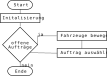
\includegraphics[scale=0.5]{src/greedy-diagram}
    \caption{Ablauf Greedy Ansatz}
    \label{figure:greedy-diagram}
\end{figure}

Im ersten Schritt wird das Fahrtzeug mit der geringsten Distanz zu seinem Ziel gewählt
(hat es kein Ziel ist die Distanz \num{0}) und alle Fahrzeuge um diese Distanz bewegt.
Dann wird geprüft, ob ihre jeweiligen Aufträge nun erfüllt sind.

Im nächsten Schritt wird für alle Fahrzeuge, welche keinen aktiven Auftrag haben, ein
nächster Auftrag ausgewählt. Dieser Schritt unterscheidet sich von dem vorherigen Ansatz,
da hier nun neben der Distanz zwischen Start- und Zielposition des Auftrags auch das
Vorhandensein eines Anschlussauftrags als Parameter für die Heuristik herangezogen wird.
Dadurch wird an der aktuellen Maschine ein Auftrag ausgewählt, welcher an seinem Ziel
einen Folgeauftrag hat. Sollte es keine Aufträge an der aktuellen Maschine geben, wird
die nächste Maschine angesteuert, welche noch Aufträge hat.

\subsubsection{Verbesserte Heuristik}
Während der Implementation der Strategie hatte sich gezeigt, dass eine Optimierung der
Heuristik möglich ist. Hierfür wurde diese wie folge angepasst:

Statt einfach nur danach zu sortieren, ob ein Auftrag einen Folgeauftrag hat, wird ein
Auftrag nach der Anzahl möglicher Folgeaufträge bewertet. Ein Auftrag, an dessen Ziel
mehr Folgeaufträge warten, hat eine höhere Priorität. Sollte es trotzdem noch mehrere
Aufträge mit der selben Priorität geben, werden diese noch einmal nach der Distanz des
Auftrags sortiert. Bei gleicher Anzahl Folgeaufträge wird der Auftrag mit der kürzesten
Distanz zwischen Start- und Zielposition gewählt.

Im weiteren Fall, dass eine Maschine keine Aufträge mehr hat, wird nicht mehr die nächste
Maschine angefahren, sondern die Maschine mit den meisten offenen Aufträgen. Sollte es
hiervon Mehrere geben, wird die Maschine gewählt, zu der aktuell kein anderes Fahrzeug
unterwegs ist.


\subsection{Implementierung}
Der Ansatz wurde mittels \emph{Python} implementiert, die Umsetzung erfolgte größtenteils
mit den mitgelieferten Paketen, einzig das \emph{numpy} Paket wurde zusätzlich verwendet
um die Berechnung der Distanzen zu vereinfachen.

Im ersten Schritt werden die Maschinen erzeugt. Diese werden als einfache Tupel ihrer
Koordinaten in einer Liste repräsentiert. Der Listenindex entspricht der \emph{ID} der
Maschine. Des Weiteren werden die Transportaufträge eingelesen und die Fahrzeuge
erstellt. Diese werden als Objekte mit folgenden Attributen repräsentiert: \emph{ID},
\emph{Position}, \emph{Ziel}, \emph{Distanz zum Ziel} und, ob sie \emph{Ladung}
transportieren.

Danach werden in einer \code{WHILE}-Schleife die Aufträge abgearbeitet. Dies erfolgt,
indem das Fahrzeug mit der kürzesten Distanz zum Ziel ermittelt wird, alle Fahrzeuge
um diese Distanz bewegt werden und alle aktiven Aufträge auf Erfüllung geprüft werden.
Alle Fahrzeuge, welche nun keinen aktiven Auftrag mehr haben, werden mit einem neuen
Auftrag versorgt. Dazu werden die oberen Heuristiken verwendet.

Dem Fahrzeug wird ein neues Ziel zugewiesen. Sollte eine Fahrt mit Ladung erfolgen, wird
dies im Fahrzeug gespeichert. Des Weiteren wird für die spätere Ausgabe der Pfade die
Fahrt des Fahrzeugs der Ausgabeliste hinzugefügt.

\subsubsection{Verbesserte Version}
Um die verbesserte Heuristik zu Implementieren wurde die Implementierung der Fahrzeuge,
Aufträge und Maschinen verändert. Für all diese Objekte wurden Klassen entworfen und
Teile der Logik als Klassenmethoden implementiert. Besonders die Implementierung der
Fahrzeuge wurde angepasst, sodass jedes Fahrzeug nun eine Liste an aktuellen Aufträgen
enthält, sowie eine Liste aller erledigter Aufträge.

Ein wichtiger Unterschied zur vorhergehenden Version ist das Speichern eines
Folgeauftrages im Falle eines Maschinenwechsels. Ein Fahrzeug, welches von einer
Maschine ohne offenen Aufträge zu einer anderen Maschine unterwegs ist, blockt bereits
den dortigen Folgeauftrag.

Somit wird der Fall umgangen, dass ein Fahrzeug zu einer Maschine fährt um dort einen
Auftrag anzunehmen, jedoch ein anderes Fahrzeug schneller war und den Auftrag bereits
angenommen hat. Dies würde sonst zu einer unnötigen Leerfahrt führen.

Erfolgte Fahrten werden nun direkt im Fahrzeug gespeichert. Somit wird am Ende für die
Ausgabe über die Fahrzeuge iteriert und die Liste ihrer Pfade direkt aus der jeweiligen
Fahrzeugliste extrahiert.


\subsection{Ergebnisse}
Aufgrund des Greedy-Ansatzes liefert das Skript die Ergebnisse ohne spürbare Verzögerung.
Gemessen wurde eine Ausführungszeit von $\approx \SI{0.205}{\second}$
für die erste Version, respektive $\approx \SI{0.251}{\second}$ für die Verbesserte.

Die Lösungsgüte ist in Tabelle \ref{table:greedy-paths} abgebildet:
\begin{table}[H]
    \centering
    \begin{tabularx}{\textwidth}{|*{4}{Y|}}
        \hline
        \multirow{2}{*}{Anzahl Fahrzeuge} & \multicolumn{2}{c|}{Berechneter Wert}\\
                                            \cline{2-3} &Version 1 &Version 2 \\
        \hline
        1    & \num{7757.18}   & \num{7165.10}    \\ \hline
        3    & \num{2612.26}   & \num{2425.26}    \\ \hline
        5    & \num{1577.01}   & \num{1462.75}    \\ \hline
    \end{tabularx}
    \caption{Ergebnisse des Greedy-Ansatzes}
    \label{table:greedy-paths}
\end{table}

\section{Ansatz 3: Ruin and Recreate}
\subsection{Strategie}
Ein weiterer Ansatz zur Berechnung eines möglichst optimalen Ablaufplans ist die
Verwendung der \emph{Ruin-and-Recreate}-Strategie beschrieben durch Schrimpf et al.
\cite{schrimpf} Dieser Algorithmus verwendet einen iterativen Ansatz, in dem zuerst Teile
der Lösung entfernt (Ruin-Schritt) und nachfolgend wieder anders zusammengesetzt
(Recreate-Schritt) werden. Bei der erneuten Zusammensetzung der Lösung wird dabei ein
Ergebnis präferiert, welches eine beschriebene Zielfunktion maximiert - in unserem
Anwendungsfall also eine Lösung, die die zurückgelegte Strecke aller Fahrzeuge (und damit
die Gesamtausführungszeit des Ablaufplans) minimiert.

\subsection{Implementierung}
Zur Implementation dieser Meta-Heuristik verwenden wir das Java-Framework jSprit, welches
auf dem von Schrimpf et al beschriebenen Grundalgorithmus basiert. Dazu werden unsere
bereitgestellten Fahrzeuge durch Objekte der Klasse \code{Vehicle} dargestellt. Diese
werden mit einer Gesamtkapazität von \num{1} erstellt und initial an den
korrespondierenden Maschinen positioniert. Die Transportanforderungen aus
\emph{transport\_demand.txt} werden in jSprit als Objekte der Klasse \code{Shipment}
abgebildet.

Jedes \code{Shipment} hat eine Größe von \num{1}, es werden also gegebenenfalls mehrere
Shipments mit der gleichen Start- und Zielposition erstellt, wenn die
Transportanforderungen dies vorgeben. Zusätzlich werden dem Algorithmus noch
benutzerdefinierte Constraints vorgegeben, die eine Senkung der maximalen Transportzeit
im Recreate-Schritt des Algorithmus bevorzugen. Der Algorithmus wird dann mit einer
Obergrenze von \num{2000} Iterationen gestartet.

\subsection{Ergebnisse}
Die Laufzeit des Programms ist direkt abhängig von der Obergrenze der Iterationen. Bei
der gesetzten Obergrenze von \num{2000} Iterationen terminiert das Programm nach
$\approx \SI{133.099}{\second}$.

Die Lösungsgüte ist in Tabelle \ref{table:ruin-and-recreate} abgebildet:
%
\begin{table}[H]
    \centering
    \begin{tabular}{|c|c|}
    \hline
    Anzahl Fahrzeuge & Berechneter Wert \\ \hline
    1                & \num{6995.31}    \\ \hline
    3                & \num{2324.02}    \\ \hline
    5                & \num{1389.65}    \\ \hline
    \end{tabular}
    \caption{Ergebnisse ruin-and-recreate}
    \label{table:ruin-and-recreate}
\end{table}

\section{Ergebnisdiskussion}
Der erste und zweite Ansatz basieren jeweils auf einem Greedy-Ansatz, daher wird bei
jeder Station der in diesem Moment beste Auftrag ausgewählt. Dies hat den Vorteil, dass
sich beide Strategien theoretisch dynamisch an neue Aufträge anpassen können. Somit
könnten während der Fahrt neue Aufträge hinzugefügt oder entfernt werden. Dies birgt
jedoch auch den Nachteil, dass diese Strategien keine optimale Lösung bieten.

Im Vergleich dazu zeigt die dritte Strategie eine deutlich bessere Lösungsgüte,
jedoch wiederum mit dem Nachteil, dass eine vorherige Berechnung stattfinden muss und eine
Veränderung der Aufträge eine Neuberechnung zur Folge hätte.

Somit hängt es vom Anwendungsfall ab, ob eine Berechnung im Voraus ausreichend ist oder
ob ein Kompromiss bei der Lösungsgüte eingegangen werden möchte.
Vergleicht man die Ergebnisse, so erkennt man in der Gegenüberstellung
\ref{table:compare-strategies}, dass der erste Greedy-Ansatz kaum eine Verbesserung
gegenüber dem Kürzeste-Distanz Ansatz bringt.
Jedoch die verbesserte Version beiden deutlich überlegen ist.
Der \emph{Ruin-and-Recreate}-Ansatz ist noch um $\approx \SI{3.85}{\percent}$ besser als
der zweite Greedy-Ansatz, jedoch auf Kosten einer um $\approx \SI{530}{\percent}$ höheren
Laufzeit.

\begin{table}[H]
    \centering
    \begin{tabular}{|c|r|r|r|}
    \hline\centering
    Strategie & \multicolumn{1}{c|}{1} & \multicolumn{1}{c|}{2.1} & \multicolumn{1}{c|}{2.2}
                                                                                        \\ \hline
    1         & 0                      & -                        & -                   \\ \hline
    2.1       & \SI{ 1.83}{\percent}   & 0                        & -                   \\ \hline
    2.2       & \SI{ 9.04}{\percent}   & \SI{ 7.35}{\percent}     & 0                   \\ \hline
    3         & \SI{12.53}{\percent}   & \SI{10.91}{\percent}     & \SI{3.85}{\percent} \\ \hline
    \end{tabular}
    \caption{Verbesserung der Ergebnisse, gemittelt aus den Verbesserungen der jeweiligen
    Ergebnissen (ein, drei und fünf Fahrzeuge).}
    \label{table:compare-strategies}
\end{table}

\chapter{Aufgabe 2}
\section{Initiale Probleme}
Bei der Umsetzung von Aufgabe 2 wurde zur Programmierung von der hauseigenen Lego Software
abgesehen. Leider wollte uns die Benutzung des \code{repeat until}-Blockes, welcher eine
\code{while}-Schleife abbilden soll, nicht gelingen. Sowohl die Bedingung $x < y$ als auch
$x > y$ führten nicht zum gewünschten Verhalten. Nur bei $x = y$ zeigte der Roboter eine
Reaktion.

Da das Programm die Rotation der Motoren allerdings in zu großen Abständen abtastet,
wurde nie exakt die 2-Meter-Marke gemessen und somit überfahren. Aufgrund dessen wurde
nach einer Alternative gesucht. Der Hinweis der Tutoren, die alte Softwareversion zu
benutzen, erreichte uns leider zu spät.

Das \emph{MicroPython\,Package}, welches ebenfalls von Lego bereitgestellt wird, bot
sich hierfür bestens an. Außerdem ermöglichte es eine einfachere Einarbeitung durch
Python-Vorkenntnisse, verständlicheren Code und Kollaboration durch Verwendung von Git.


\section{Experiment 1: Freie Fahrt}
\subsection{Aufgabenstellung}
Das Fahrzeug soll ohne weitere Sensorik eine Strecke von $\SI{2}{\m}$ geradeaus
zurücklegen.

\subsection{Herangehensweise}
Die Geschwindigkeit des Motors setzen wir initial auf $\SI{440}{\frac{\mm}{\s}}$, da dies
scheinbar die Maximalgeschwindigkeit ist. Um die zurückgelegte Strecke des Roboters zu
ermitteln, muss die Rotation des Motors gemessen werden. Mit Hilfe der Funktion
\code{motor.angle()} wird die Motorstellung in Grad ausgelesen und kann mit Hilfe des
Radumfangs $d$ in eine Strecke umgerechnet werden.

\begin{equation}
    \label{equation:2meterstrecke}
    \begin{aligned}
       d &= \SI{56}{\mm}\\
       u &= \pi \cdot d \approx \SI{176}{\mm} \\
       y &= \frac{\SI{2}{\m}}{u} \cdot \SI{360}{\degree} \approx \SI{4092.6}{\degree}
    \end{aligned}
\end{equation}

Nach Gleichung \ref{equation:2meterstrecke} entsprechen 2 Meter also ca.
\SI{4092.6}{\degree}.

\subsection{Herausforderungen bei der Problemstellung}
Leider mussten wir feststellen, dass der errechnete Werte stark von der Realität abweicht.
Nach einigen Testläufen haben wir den Wert manuell auf $y = \SI{3870}{\degree}$ eingestellt.
Wir ließen den Roboter mehrmals die Strecke abfahren und ermittelten dabei die benötigte
Zeit. Diese misst der Roboter selbst und gibt sie auf dem Display aus, um mögliche
Messfehler unsereseits zu vermeiden. Außerdem maßen wir die Abweichung von der
erwarteten Zielposition. Dies unterteilten wir in zwei Messreihen: Abweichung in der
Länge, also ob der Roboter zu kurz oder übers Ziel hinaus gefahren ist. Und Abweichung in
der Breite, also ob der Roboter nach links oder rechts lenkt.

\subsection{Auswertung}
\subsubsection{Abweichung vom Gradmaß}
Es gibt verschiedene Gründe für die Abweichung zwischen dem berechnetem und gemessenem
Gradmaß. Dazu zählen Messfehler sowohl beim Aufbau der Testumgebung als auch bei der
Ermittlung des Raddurchmessers. Durch das Gewicht des Roboters kann außerdem der Reifen
zusammengedrückt werden, was zu einer Veränderung des Raddurchmessers führt. Weiterhin
erfolgt das Bremsen des Roboters nicht durch aktives Abbremsen, sondern durch Ausrollen
der Motoren. Dadurch schaltet der Roboter beim Erreichen der gewünschten Radrotation
$y$ zwar die Motoren ab, kommt jedoch erst ein paar Zentimeter später zum Stehen.
Letztlich können auch Fehler bei der Startaufstellung des Roboters, wie beispielsweise
Über- oder Unterschreiten der Startlinie und der initialen Stellung des Hinterrads
auftreten.

\subsubsection{Zeitmessung}
Tabelle \ref{table:zeitmessung} zeigt die Messergebnisse der Zeitmessung. Die Streuung ist
sehr klein.
Abbildung \ref{figure:zeitverteilung} zeigt in einem Histogramm die Verteilung der
Daten im Vergleich zu einer Normalverteilung. Mit grafischer Analyse könnte man eine
leichte Annäherung an die Verteilung festellen.
%
\begin{table}[H]
    \centering
    \begin{tabular}{|c|c|}
    \hline
    Mean               & $\SI{5,335}{\s}$ \\ \hline
    Standardabweichung & $\SI{0,013}{\s}$ \\ \hline
    Min                & $\SI{5,31}{\s}$ \\ \hline
    Max                & $\SI{5,36}{\s}$ \\ \hline
    \end{tabular}
    \caption{Zeitmessung}
    \label{table:zeitmessung}
\end{table}
%
\begin{figure}[H]
    \centering
    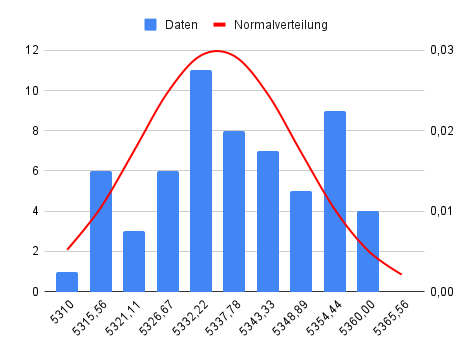
\includegraphics[scale=0.5]{src/charts/zeitverteilung.png}
    \caption{Zeitverteilung}
    \label{figure:zeitverteilung}
\end{figure}
%
\subsubsection{Längenabweichung}
Tabelle \ref{table:laengenabweichung} stellt die Abweichung von der erwarteten
Zielposition in der Länge dar. Ein optimales Ergebnis wird hier mit $\SI{0}{\mm}$
repräsentiert, während negative Werte für zu kurze Fahrten und positive Werte für zu
lange Fahrten stehen. Den stärksten Fehlereinfluss auf die Streuung hier hat
wahrscheinlich die Variation der initiale Startposition des Roboters.
%
\begin{table}[H]
    \centering
    \begin{tabular}{|c|c|}
    \hline
    Mean               & $\SI{-10,18}{\mm}$ \\ \hline
    Standardabweichung & $\SI{3,24}{\mm}$ \\ \hline
    Min                & $\SI{-19}{\mm}$ \\ \hline
    Max                & $\SI{-3}{\mm}$ \\ \hline
    \end{tabular}
    \caption{Längenabweichung}
    \label{table:laengenabweichung}
\end{table}
%
Die Verteilung der Daten, wie im Histogramm in Abbildung \ref{figure:laengenverteilung}
zu sehen, lässt auf eine annähernde Normalverteilung der Messwerte schließen. Diese
Erkenntnis kann genutzt werden, um den Roboter erneut zu kalibrieren. Solch eine kleine
Abweichung konnte bei der initialen Kalibrierung nur schwer bemerkt werden, summiert sich
allerdings bei hoher Anzahl an Fahrten auf uns sorgt für Probleme und Ineffizienzen.
%
\begin{figure}[H]
    \centering
    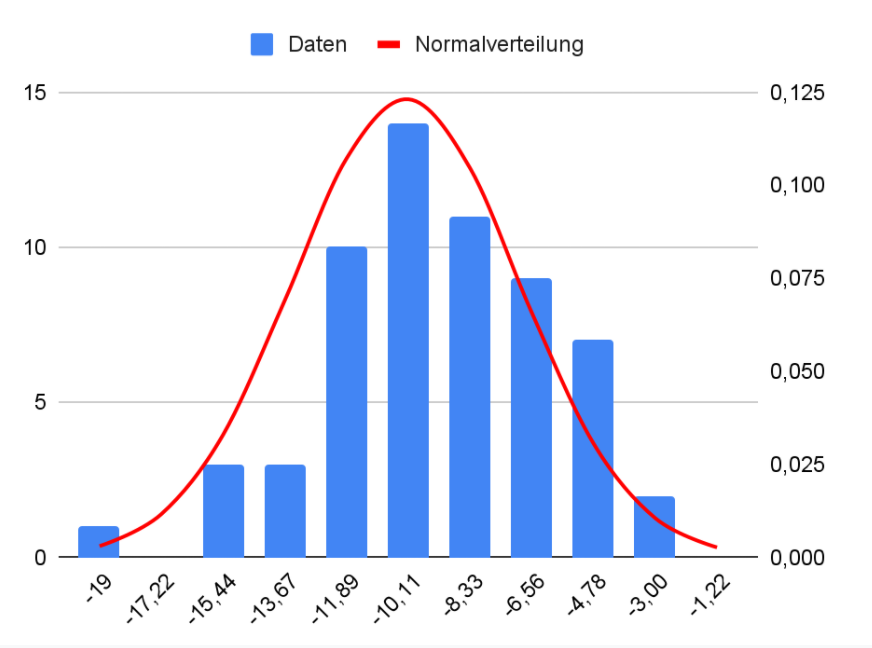
\includegraphics[scale=0.5]{src/charts/laengenverteilung.png}
    \caption{Längenverteilung}
    \label{figure:laengenverteilung}
\end{figure}
%
\subsubsection{Breitenabweichung}
Tabelle \ref{table:breitenabweichung} stellt die Abweichung von der erwarteten
Zielposition in der Breite dar. Ein optimales Ergebnis wird wieder mit $\SI{0}{\mm}$
repräsentiert, während negative Werte für eine Linkslenkung und positive Werte für eine
Rechtslenkung stehen.
%
\begin{table}[H]
    \centering
    \begin{tabular}{|c|c|}
    \hline
    Mean               & $\SI{-35,98}{\mm}$ \\ \hline
    Standardabweichung & $\SI{31,15}{\mm}$ \\ \hline
    Min                & $\SI{-121}{\mm}$ \\ \hline
    Max                & $\SI{25}{\mm}$ \\ \hline
    \end{tabular}
    \caption{Breitenabweichung}
    \label{table:breitenabweichung}
\end{table}
%
Auch im Histogramm in Abbildung \ref{figure:breitenverteilung} lässt sich eine
Normalverteilung der Messwerte erkennen. Wie auch bei der Längenabweichung kann diese
Erkenntnis zur nachträglichen Kalibrierung genutzt werden. 
%
\begin{figure}[H]
    \centering
    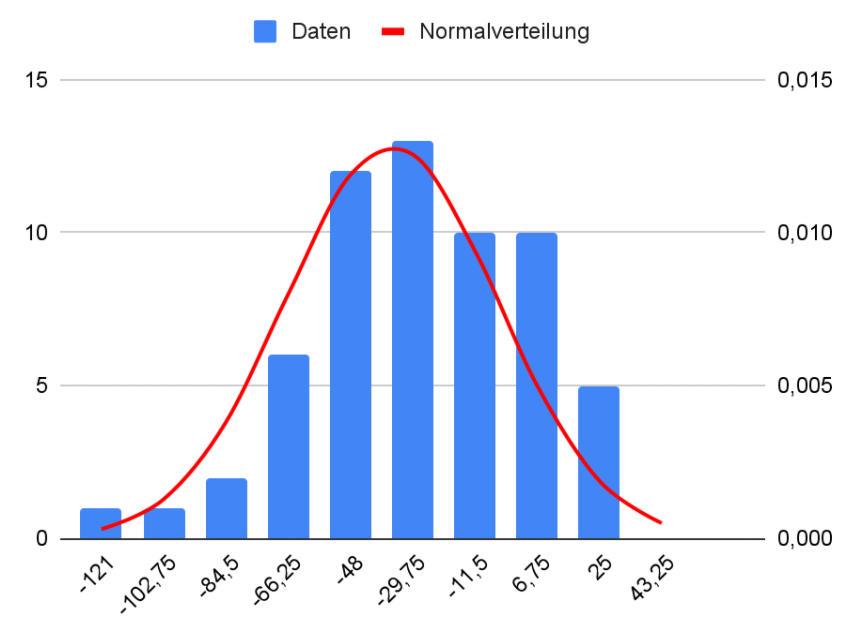
\includegraphics[scale=0.5]{src/charts/breitenverteilung.png}
    \caption{Längenverteilung}
    \label{figure:breitenverteilung}
\end{figure}
Es liegen höchstwahrscheinlich die selben Gründe für Abweichung vor. Allerdings ist eine
stärkere Streuung zu erkennen. 

\subsubsection{Zusammenhang Längen- und Breitenabweichung}
Begründet werden kann diese Streuung mit dem Verhältnis von Längen- und Breitenabweichung. 
Mathematisch gesehen führt eine Abweichung von $\SI{100}{\mm}$ zu einer Fahrtstrecke von
$\SI{2002,5}{\mm}$, bevor der Roboter die Ziellinie überquert. Dabei wird eine gerade
Strecke angenommen. Da der Roboter per Programmierung nur 2 Meter zurückgelegt, führt das
zu einer Längenabweichung von $\SI{2,5}{\mm}$. Das Verhältnis von Längen- zu
Breitenabweichung würde also $1:40$ betragen. Sollte einer der Motoren weniger Leistung
als der andere liefern, führt das zu einer Kurvenfahrt. Dies könnte man überprüfen, indem
man Messwerte auf halber Strecke, oder noch öfter, ermittelt oder indem man das
mathematische Verhätnis mit dem Verhätnis der beiden Mittelwerte der Messreihen
vergleicht. Dieses beträgt circa $1:3,6$. Der Roboter legt also mehr Strecke zurück, also
er rechnerisch fahren müsste. Womöglich ist das eine Anzeichen für eine Kurvenfahrt und
damit ungleich starke Motoren, allerdings spielen wahrscheinlich auch hier Messfehler und
ein ungenauer Versuchsaufbau eine signifikante Rolle. Abbildung 
\ref{figure:verhaeltnis_laenge_breite} zeigt das Verhältnis der Messergebnisse von Länge
und Breite.
%
\begin{figure}[H]
    \centering
    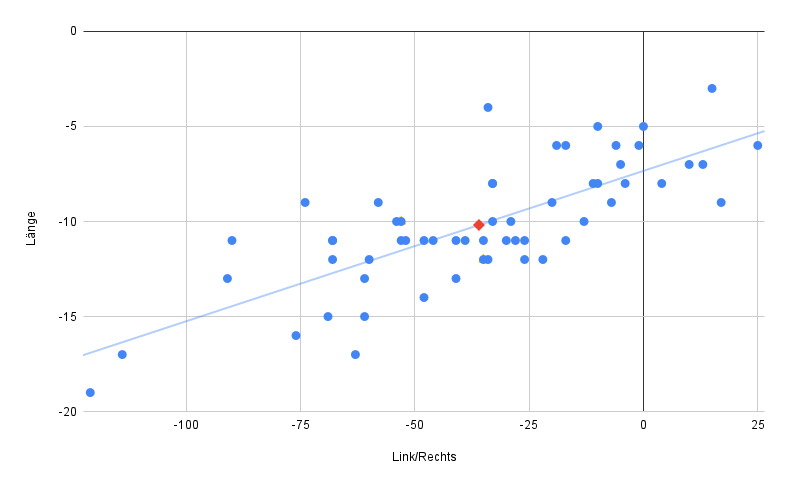
\includegraphics[scale=0.5]{src/charts/verhaeltnis_laenge_breite.png}
    \caption{Verhältnis Länge und Breite}
    \label{figure:verhaeltnis_laenge_breite}
\end{figure}
%

\subsubsection{Zusammenhang örtliche und zeitliche Abweichung}
Da man aber annehmen kann, dass sich die Startposition über viele Versuche hinweg mittelt,
wird klar, dass der Roboter womöglich einen leichten Linksdrall hat. Auch das kann bei der
Kalibrierung berücksichtigt werden. Möglicherweise liegt aber auch ein technischer Defekt oder
Verschleiß vor. Des Weiteren besteht trotz Kalibrierung eine große Streuung. Diese kann
theoretisch nur zwei Gründe haben. Entweder haben die Motoren zwischen den
Messdurchläufen Leistungsschwankungen oder der Roboter fährt eine relativ konstante,
wenn u.U. auch gebogene, Linie und die Startposition und/oder das Anfahren sorgen für die
gemessene Streuung. Sollte Ersteres der Fall sein, müssten wir eine Korrelation zwischen
Breitenabweichung und Zeit festellen, da wir das Erreichen des Ziels an der Umdrehung des
linken Rades fest machen. Ein Durchlauf mit niedriger Performance dieses Rades hätte eine
längere Fahrtzeit zur Folge. Wie Abbildung \ref{figure:verhaeltnis_zeit_breite} allerdings
zeigt, lässt sich solch eine Korrelation, zumindest über die 60 Versuchsdurchläufe
hinweg, nicht feststellen. Also geht die Streuung vermutlich wieder aus den bekannten
Messungs- und Aufbauungenauigkeiten hervor. Diesen kann ausschließlich entgegen gewirkt
werden, indem der Roboter sich per Sensorik an der Linie orientiert (siehe: Experiment 2). 
%
\begin{figure}[H]
    \centering
    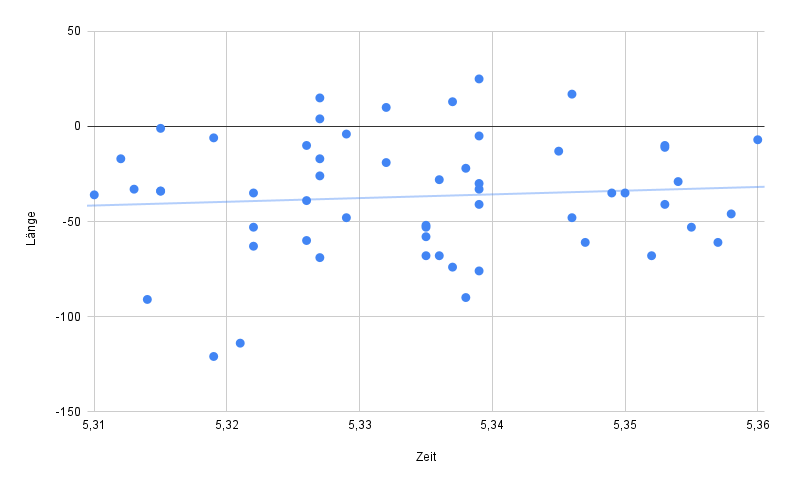
\includegraphics[scale=0.5]{src/charts/verhaeltnis_breite_zeit.png}
    \caption{Verhältnis Zeit- und Breitenabweichung}
    \label{figure:verhaeltnis_zeit_breite}
\end{figure}
%
\section{Experiment 2: Folgen einer Spur}
\subsection{Aufgabenstellung}
Das Fahrzeug soll mit seiner Sensorik eine Strecke von $\SI{2}{\m}$ geradeaus
zurücklegen.

\subsection{Herangehensweise}
Für diese Aufgabe muss der Farbsensor des Roboters einbezogen werden. Um die Messwerte
des Sensors in die Programmierung des Roboters mit einzubeziehen, wurde ein
Proportional-Controller genutzt. Ein PID-Controller würde vermutlich für kaum merkbare
Verbesserung sorgen, steigert die Komplexität allerdings extrem. Damit der Farbsensor
möglichst aussagekräftige und unterscheidbare Werte liefert, nutzen wir weißes Tape auf
einem schwarzen Tisch, was für starke Kontraste sorgt.

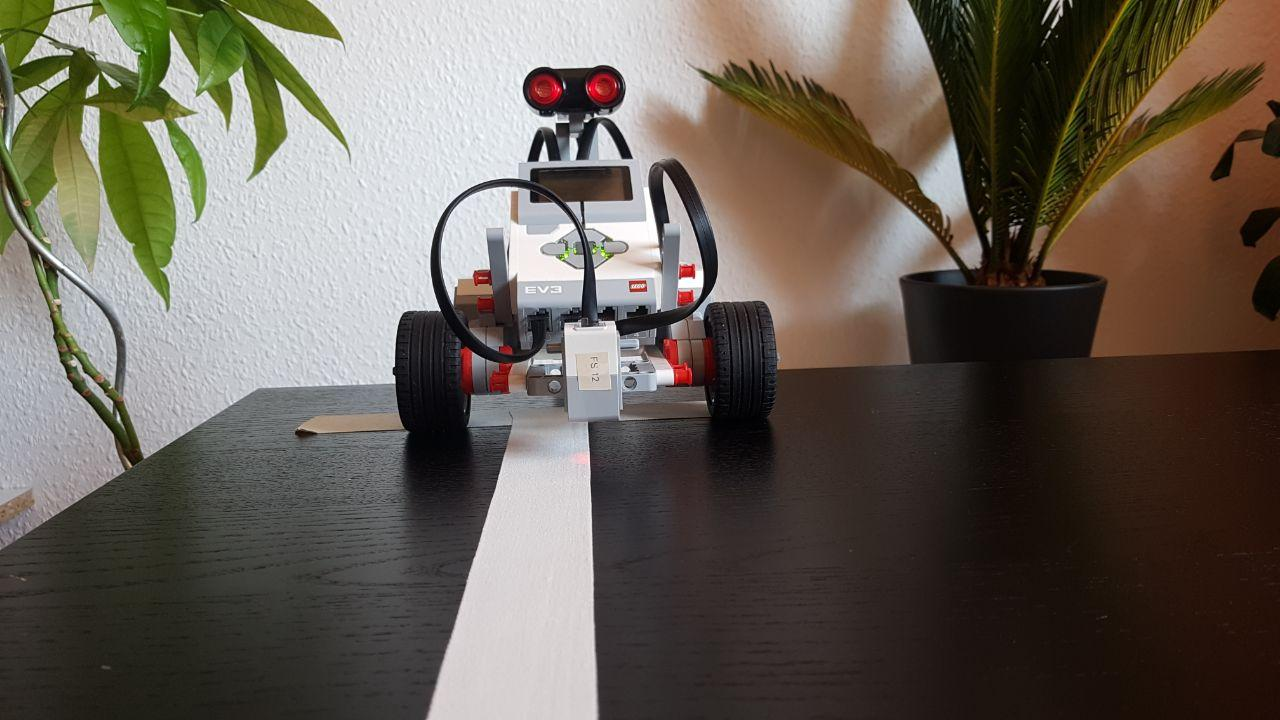
\includegraphics[scale=0.5]{src/images/robot_front.jpg}

\subsection{Herausforderungen bei der Problemlösung}
Die größte Schwierigkeit bei dieser Aufgabe besteht in der Kalibrierung des P-Controllers.
Allerdings lässt sich bei nur einer Regelgröße relativ schnell ein geeigneter Parameter
finden. Ein weiteres Problem stellt der Lichteinfall dar. Durch Sonneneinstrahlung oder
Lampenreflektion könnten die Sensormesswerte verfälscht werden. Am besten lässt sich das
Experiment vermutlich im Dunkeln durchführen, da der Sensor sein eigenes Licht mitbringt.
Bereits genannte Gründe für Abweichung kommen auch hier wieder zum tragen, wobei der
Roboter Ungenauigkeiten in der Startposition relativ schnell kompensieren kann.

\subsection{Auswertung}
Tabelle \ref{table:zeitmessung2} zeigt die Ergebnisse der Zeitmessung. Bereits nach 10
Testdurchläuften stellen wir fest, dass die Abweichungen von der erwarteten Zielposition
minimal und teilweise nicht messbar waren, weshlab wir uns von weiteren Durchläufen keine
neuen Erkenntnisse erwarteten. Der Roboter profitiert also sehr stark von seinem
Farbsensor und dem P-Regler. Eine leichte Verschlechterung der Zeitenmessung lässt sich 
dennoch festellen. Das Minimum ist kleiner, da der Roboter in diesem Durchlauf vermutlich
sehr gute Startbedingungen hatte und eine perfekte Linie fahren konnte. Dennoch sind
Mittelweit, Streuung und Maximum größer. Hier spielen höchstwahrscheinlich die stetigen
Nachbesserungen des Reglers eine große Rolle. Dennoch ist der Zeitverlust im Vergleich
zum Präzisionsgewinn minimal und eine solche Roboterkonfiguration lohnt sich definitiv.
%
\begin{table}[H]
    \centering
    \begin{tabular}{|c|c|c|}
    \hline
                       & Experiment 1      & Experiment 2      \\ \hline
    Mean               & $\SI{5,335}{\mm}$ & $\SI{5,343}{\mm}$ \\ \hline
    Standardabweichung & $\SI{0,013}{\mm}$ & $\SI{0,074}{\mm}$ \\ \hline
    Min                & $\SI{5,31}{\mm}$  & $\SI{5,225}{\mm}$ \\ \hline
    Max                & $\SI{5,36}{\mm}$  & $\SI{5,471}{\mm}$ \\ \hline
    \end{tabular}
    \caption{Zeitmessung}
    \label{table:zeitmessung2}
\end{table}

\section{Experiment 3: Umfahren eines Hindernisses}
\subsection{Aufgabenstellung}
Das Fahrzeug soll mit Hilfe seiner Sensorik eine definierte Strecke abfahren und dabei ein
fiktives Hindernis umfahren.

\subsection{Herangehensweise}
Theoretisch besitzt der Roboter bereits alle nötigen Fähigkeiten, um auch einer
abbiegenden Linie zu folgen. Allerdings würde ihn die Geschwindigkeit aus der Bahn werfen.
Zu testen wäre also die größtmögliche Geschwindigkeit, bei der der Kurs verlässlich
abgefahren werden kann. Diese Geschwindigkeit kann dann mit dem Erweitern des P-Controller
zu einem PID-Controller verbessert werden.

\subsection{Herausforderungen bei der Problemlösung}
Die richtigen Parameter für einen PID-Controller zu finden stellt sich als äußerst
komplex dar. Scheinbar gibt es dabei auch keine Best-Practices sondern man muss einfach
probieren. \enquote{Verlässliche Einstellungen} des Roboters definieren wird so, dass er
den Kurs zehn mal in Folge erfolgreich absolvieren muss.

\subsection{Auswertung}
Für die Testläufe mit dem P-Controller erreichten wir eine maximale Geschwindigkeit
von $\SI{100}{\frac{\mm}{\s}}$. Diese konnten wir mit dem PID-Controller auf
$\SI{140}{\frac{\mm}{\s}}$ verbessern. Der Roboter absolvierte auch einzelne Testläufe
mit höheren Geschwindigkeiten erfolgreich, jedoch nicht zuverlässig.

Tabelle \ref{table:zeitmessung3} enthält die Ergebnisse der Zeitmessung, auch hier
liegen die Messergebnisse wieder stark beieinander. Allerdings unterscheiden sie sich,
wie erwartet, stark von den vorherigen Experimenten. Der Mittelweit ist circa 2,5 und die
Standardabweichung 1,6 mal größer.
%
\begin{table}[H]
    \centering
    \begin{tabular}{|c|c|c|c|}
    \hline
                       & Experiment 1      & Experiment 2      & Experiment 3       \\ \hline
    Mean               & $\SI{5,335}{\mm}$ & $\SI{5,343}{\mm}$ & $\SI{12,804}{\mm}$ \\ \hline
    Standardabweichung & $\SI{0,013}{\mm}$ & $\SI{0,074}{\mm}$ & $\SI{0,119}{\mm}$  \\ \hline
    Min                & $\SI{5,31}{\mm}$  & $\SI{5,225}{\mm}$ & $\SI{12,551}{\mm}$ \\ \hline
    Max                & $\SI{5,36}{\mm}$  & $\SI{5,471}{\mm}$ & $\SI{12,977}{\mm}$ \\ \hline
    \end{tabular}
    \caption{Zeitmessung}
    \label{table:zeitmessung3}
\end{table}
%
Weitere Optimierung sind möglich, indem man die Parameter des PID-Controllers verbessert.
Jedoch ist nicht klar, wann ein Optimum erreicht ist und kann somit unendlich viel Zeit
kosten. Des Weiteren hätte der Roboter einen Vorteil, wenn die Abbiegungen der Strecke
etwas kurviger wären oder zumindest einen stumpferen anstatt eines rechten Winkels
hätten. Leider kann der Roboter in diesem Versuchsaufbau keinen Nutzen aus seinem
Ultraschallsensor ziehen. Sollte er auf ein Hindernis zufahren, würde er dies frühzeitig
erkennen, seine Geschwindigkeit reduzieren, die Kurve sauber fahren und danach wieder
beschleunigen. Falls in einem realen Szenario kein Hindernis im Weg sein sollte, sondern
ausschließlich Einschränkungen der Route, könnte man dies dem Roboter über eine Karte,
Matrix oder einen Graphen mitteilen, sodass er ebenfalls im Voraus auf Kurven reagieren
kann.

\chapter{Aufgabe 3}
In der Aufgabenstellung werden Annahmen getroffen, welches das gesamte Konzept
simplifizieren. Im Folgenden wollen wir betrachten, welche möglichen Auswirkungen die
Realität auf das gegebene Szenario hat, wenn also diese Annahmen nicht mehr gemacht werden
können.

\section{Platzbedarf}
\begin{displayquote}
    ``Es befinden sich keine statischen oder dynamischen Hindernisse im Layout. [...]
    Die gesamte Fläche ist befahrbar. [...] Alle Fahrzeuge fahren auf direktem Weg
    zwischen den Maschinen (euklidische Distanz).'' \cite{aufgabenstellung}
\end{displayquote}
%
Ein Unternehmen, welches autonome Transportsysteme so effizient wie möglich einsetzen
möchte, wird sicherlich auch den zur Verfügung stehenden Platz in ihrer Logistikhalle
sinnvoll nutzen wollen. Flächen frei zu lassen, nur damit die Fahrzeug nicht mit
Hindernissen kollidieren können, stellt sich in den meisten Fällen wahrscheinlich aus
unökonomisch heraus. Mit dynamischen Hindernissen, z.B. andere Roboter, kann
vergleichsweise einfach gelöst werden, indem die Fahrzeuge die Positionen der anderen
Fahrzeuge übermittelt bekommen und dementsprechend reagieren können. Menschen als
dynamische Hindernisse stellen sich womöglich als größeres Problem dar. Moderne
Kamerasysteme können evtl. visuell ihre Umgebung wahrnehmen, Personen erkennen und
bremsen bzw. ausweichen, jedoch ist das mit großen Kosten für Technik verbunden und das
System muss einwandfrei funktionieren um Arbeitsunfälle zu vermeiden. Sollten
Kamerasysteme solcher Art nicht zum Einsatz kommen, gebietet der Arbeitsschutz eine
klare, mindestens visuelle Abtrennung des Bereiches für die Fahrzeuge und des begehbaren
Bereiches für Personen. Das kollidiert allerdings wiederum mit der Annahme, die gesamte
Fläche sei befahrbar. Eine mögliche Lösung wäre, das Transportsystem auf eine tiefer
oder höher liegende Ebene zu verlegen. Somit wäre zumindest die Fahrzeug- und
Personendomäne getrennt.

\section{Auftragszeit und -reihenfolge}
\begin{displayquote}
    ``Ein einzelner Auftrag hat keinen bestimmten Liefer- oder Abholzeitpunkt. [...] Die
    Aufträge sind homogen, d.h. es liegen keine geforderte Reihenfolge oder Priorisierung
    vor.'' \cite{aufgabenstellung}
\end{displayquote}
%
Bei Unternehmen, in denen 24/7 gearbeitet wird, muss der Auftragspool entweder nach einer
gewissen Zeit abgearbeitet sein und dann neu gestartet werden, was mit Overhead und damit
Ineffizienz verbunden ist. Oder die zu transportierenden Güter bekommen ein weiteres
Deadline-Attribut, welches im Scheduling-Algorithmus mit einbezogen werden muss.
Unternehmen, bei denen das nicht der Fall ist, könnten ihren Zeithorizont der Arbeitszeit
anpassen. Das bedeutet, am Ende des Tages ist der Aufgabenpool abgearbeitet. Allerdings
können dann zwischendrin keine neuen Aufträge eingepflegt werden und man kann nicht
erwarten, dass bestimmt Aufträge eher fertig werden als andere. Dafür müssten diese
Unternehmen dann ebenfalls den Auftragspool neu starten oder Prioritäten vergeben.

\section{Treibstoff und Verschleiß}
\begin{displayquote}
    ``Fahrzeuge sind zu 100\% einsatzbereit und fallen nie aus. [...] Fahrzeuge haben eine
    unendliche Reichweite, können also unendlich weit/lange fahren.''
    \cite{aufgabenstellung}
\end{displayquote}
%
Da Verschleiß und Energievorrat immer eine Rollen spielen, kommt es in der Realität
unvermeidlich zu Ausfällen. Selbst bei unseren Experimenten in Aufgabe 2 ist während der
Durchführung der Roboter wegen zu niedrigem Akkustand ausgefallen. Man kann dies natürlich
mit zusätzlicher Sensorik überwachen um rechtzeitig den Roboter zu warten. Allerdings
bedeutet das an sich schon einen Ausfall für den Roboter und ist zusätzlich mit Hardware-
und Personalkosten verbunden.

\section{Be- und Entladezeiten}
\begin{displayquote}
    ``Es fallen keine Tot-, Neben- und Handhabungszeiten an.''
    \cite{aufgabenstellung}
\end{displayquote}
%
Natürlich ist in der Realität das Be- und Entladen mit einem gewissen Zeitaufwand
verbunden. Diesen kann man allerdings minimal und über verschiedene Maschinen hinweg
gleich halten, wenn ein effizientes Be- und Entladungssystem zum Einsatz kommt.

\section{Fahrzeugkollisionen}
\begin{displayquote}
    ``Die Fahrzeuge sind dimensionslos, d.h. Es finden keine Konflikte zwischen den
    Fahrzeugen statt, womit keine Ausweichmanöver von Nöten sind.''
    \cite{aufgabenstellung}
\end{displayquote}
%
Wie die bereitgestellten Videos der Simulation gezeigt haben, ist diese Annahme weit von
der Realität entfernt. Es wurden dabei ausschließlich Beschleunigung und Dimension der
Roboter einbezogen, was bereits zu einer \SIrange{16}{65}{\percent} längeren
Bearbeitungszeit führt. Bei der Kollisionsdetektion und den Ausweichmanövern gibt es
eventuell noch etwas Verbesserungspotential. Des Weiteren könnte man einen Parameter
hinzufügen, welcher die Anzahl an Kollisionen zählt und vom Algorithmus minimiert werden
sollte. Jedoch führt eine minimal Kollisionszahl wahrscheinlich nicht immer zu besseren
Zeiten, da die Roboter dann Umwege fahren müssten.

\section{Maschinenkollisionen}
\begin{displayquote}
    ``Die Maschinen sind dimensionslos, d.h. die Fahrzeuge fahren exakt zu den
    angegebenen Koordinaten der Maschinen, um ein Transportgut aufzunehmen oder
    abzugeben.'' \cite{aufgabenstellung}
\end{displayquote}
%
Mit hoher Wahrscheinlichkeit muss der Roboter in der Realität auch mal die ein oder
andere Maschine umfahren. Wie die Erkenntnisse aus Aufgabe 2 zeigen, benötigt der Roboter
beim Umfahren von Hindernissen im Vergleich zu einer geraden Strecke mindestens das
2,5fache der Zeit. Allerdings spielt die Dimension der Maschinen bei dem gegebenen
Hallenlayout, und auch bei ähnlichen Layouts, eine relativ geringe Rolle. Die Koordinaten
sind mehr oder weniger kreisförmig angeordnet, sodass eine Kollision mit einer Maschine
womöglich vermieden werden kann, wenn sich die Roboter nur im Kreisinneren aufhalten.
Allerdings führt, wie bereits beschrieben, ein möglichst freier Raum auf den Routen der
Roboter zu großem Platzbedarf und somit erhöhten Kosten und Ineffizienzen.

\section{Beschleunigung}
\begin{displayquote}
    ``Fahrzeuge fahren durchgängig mit der maximalen Geschwindigkeit von 1
    Streckeneinheit/Zeit.'' \cite{aufgabenstellung}
\end{displayquote}
%
Aus hier gibt die Simulation Aufschluss über das Verhalten in der Realität. Wie viel des
zusätzlichen Zeitbedarfs jeweils der Beschleunigung oder dem Kollidieren der Roboter
zuzuschreiben ist, lässt sich schwer sagen. Fakt ist jedoch, das positive und negative
Beschleunigung Zeit kosten. Mit stärkerer Motorisierung und besseren Bremsen könnte dies
verbessert werden, doch auch hier spielt die Kostenabwägung eine entscheidende Rolle.
Ebenso zeigen die Ergebnisse der Experimente, dass ein Abbremsen vor dem Umfahren eines
Hindernisses zu besseren Resultaten führen würde. Das erhöht natürlich die Anzahl an
Beschleunigungsmanövern erneut und müsste mit der Gesamtzeitersparnis ins
Verhältnis gesetzt werden.

\section{Größe der Fahrzeugflotte}
Die Ergebnisse in Aufgabe 1 deuten auf eine lineare Abnahme der Zeit mit steigender
Roboteranzahl hin. Ein Fahrzeug pro Auftrag wäre also mit den getroffenen Annahmen die
optimale Lösung. Jedoch werden viele der bereits genannten Probleme mit steigender Anzahl
von Fahrzeugen verstärkt, sodass ab einer bestimmten Zahl die benötigte Zeit nicht mehr
abnimmt und unter Umständen sogar steigt. Auch die Erhöhung der Maschinenanzahl kann hier
nur bedingt Abhilfe schaffen, da sich dennoch viele Routen der Roboter kreuzen und die
Kollisionsanzahl hoch bleibt.

\bibliographystyle{unsrt}
\bibliography{bibliography}

\end{document}
